\documentclass{article}
\usepackage[paperwidth=14in, paperheight=14in, margin=0.45in]{geometry}
\usepackage{tikz}
\usepackage{amsmath}
\usepackage[T1]{fontenc}
\usepackage{lmodern}
\usepackage{float}
\usepackage{pdflscape}

\usetikzlibrary{
    arrows.meta,
    positioning,
    calc,
    fit,
    backgrounds,
    shapes.geometric
}

\pagestyle{empty}

% ------------------------------------------------------------
% Styles
% ------------------------------------------------------------

\tikzset{
    package/.style={
        draw=black,
        rounded corners=3pt,
        thick,
        fill=gray!5,
        inner sep=10pt
    },
    package title/.style={
        font=\large\bfseries,
        anchor=north west
    },
    classbox/.style={
        draw=black!75,
        rounded corners=2pt,
        fill=white,
        align=left,
        font=\small,
        text width=4.2cm,
        inner sep=6pt
    },
    wideclassbox/.style={
        draw=black!75,
        rounded corners=2pt,
        fill=white,
        align=left,
        font=\small,
        text width=5.2cm,
        inner sep=6pt
    },
    smallclass/.style={
        draw=black!75,
        rounded corners=2pt,
        fill=white,
        align=center,
        font=\small\bfseries,
        minimum width=2.5cm,
        minimum height=0.65cm,
        inner sep=5pt
    },
    relation/.style={
        -{Stealth[length=2.2mm]},
        thick
    },
    dependency/.style={
        -{Stealth[length=2.2mm]},
        thick,
        dashed
    },
    inheritance/.style={
        -{Triangle[open,length=3mm,width=3mm]},
        thick
    }
}

\begin{document}

% ============================================================
% PAGE 1: PACKAGE STRUCTURE
% ============================================================

\begin{landscape}
\begin{center}
    {\LARGE\bfseries Project Package Structure}

    \vspace{0.25cm}
    {\small Primary classes and responsibilities by Python module}
\end{center}

\vspace{0.25cm}

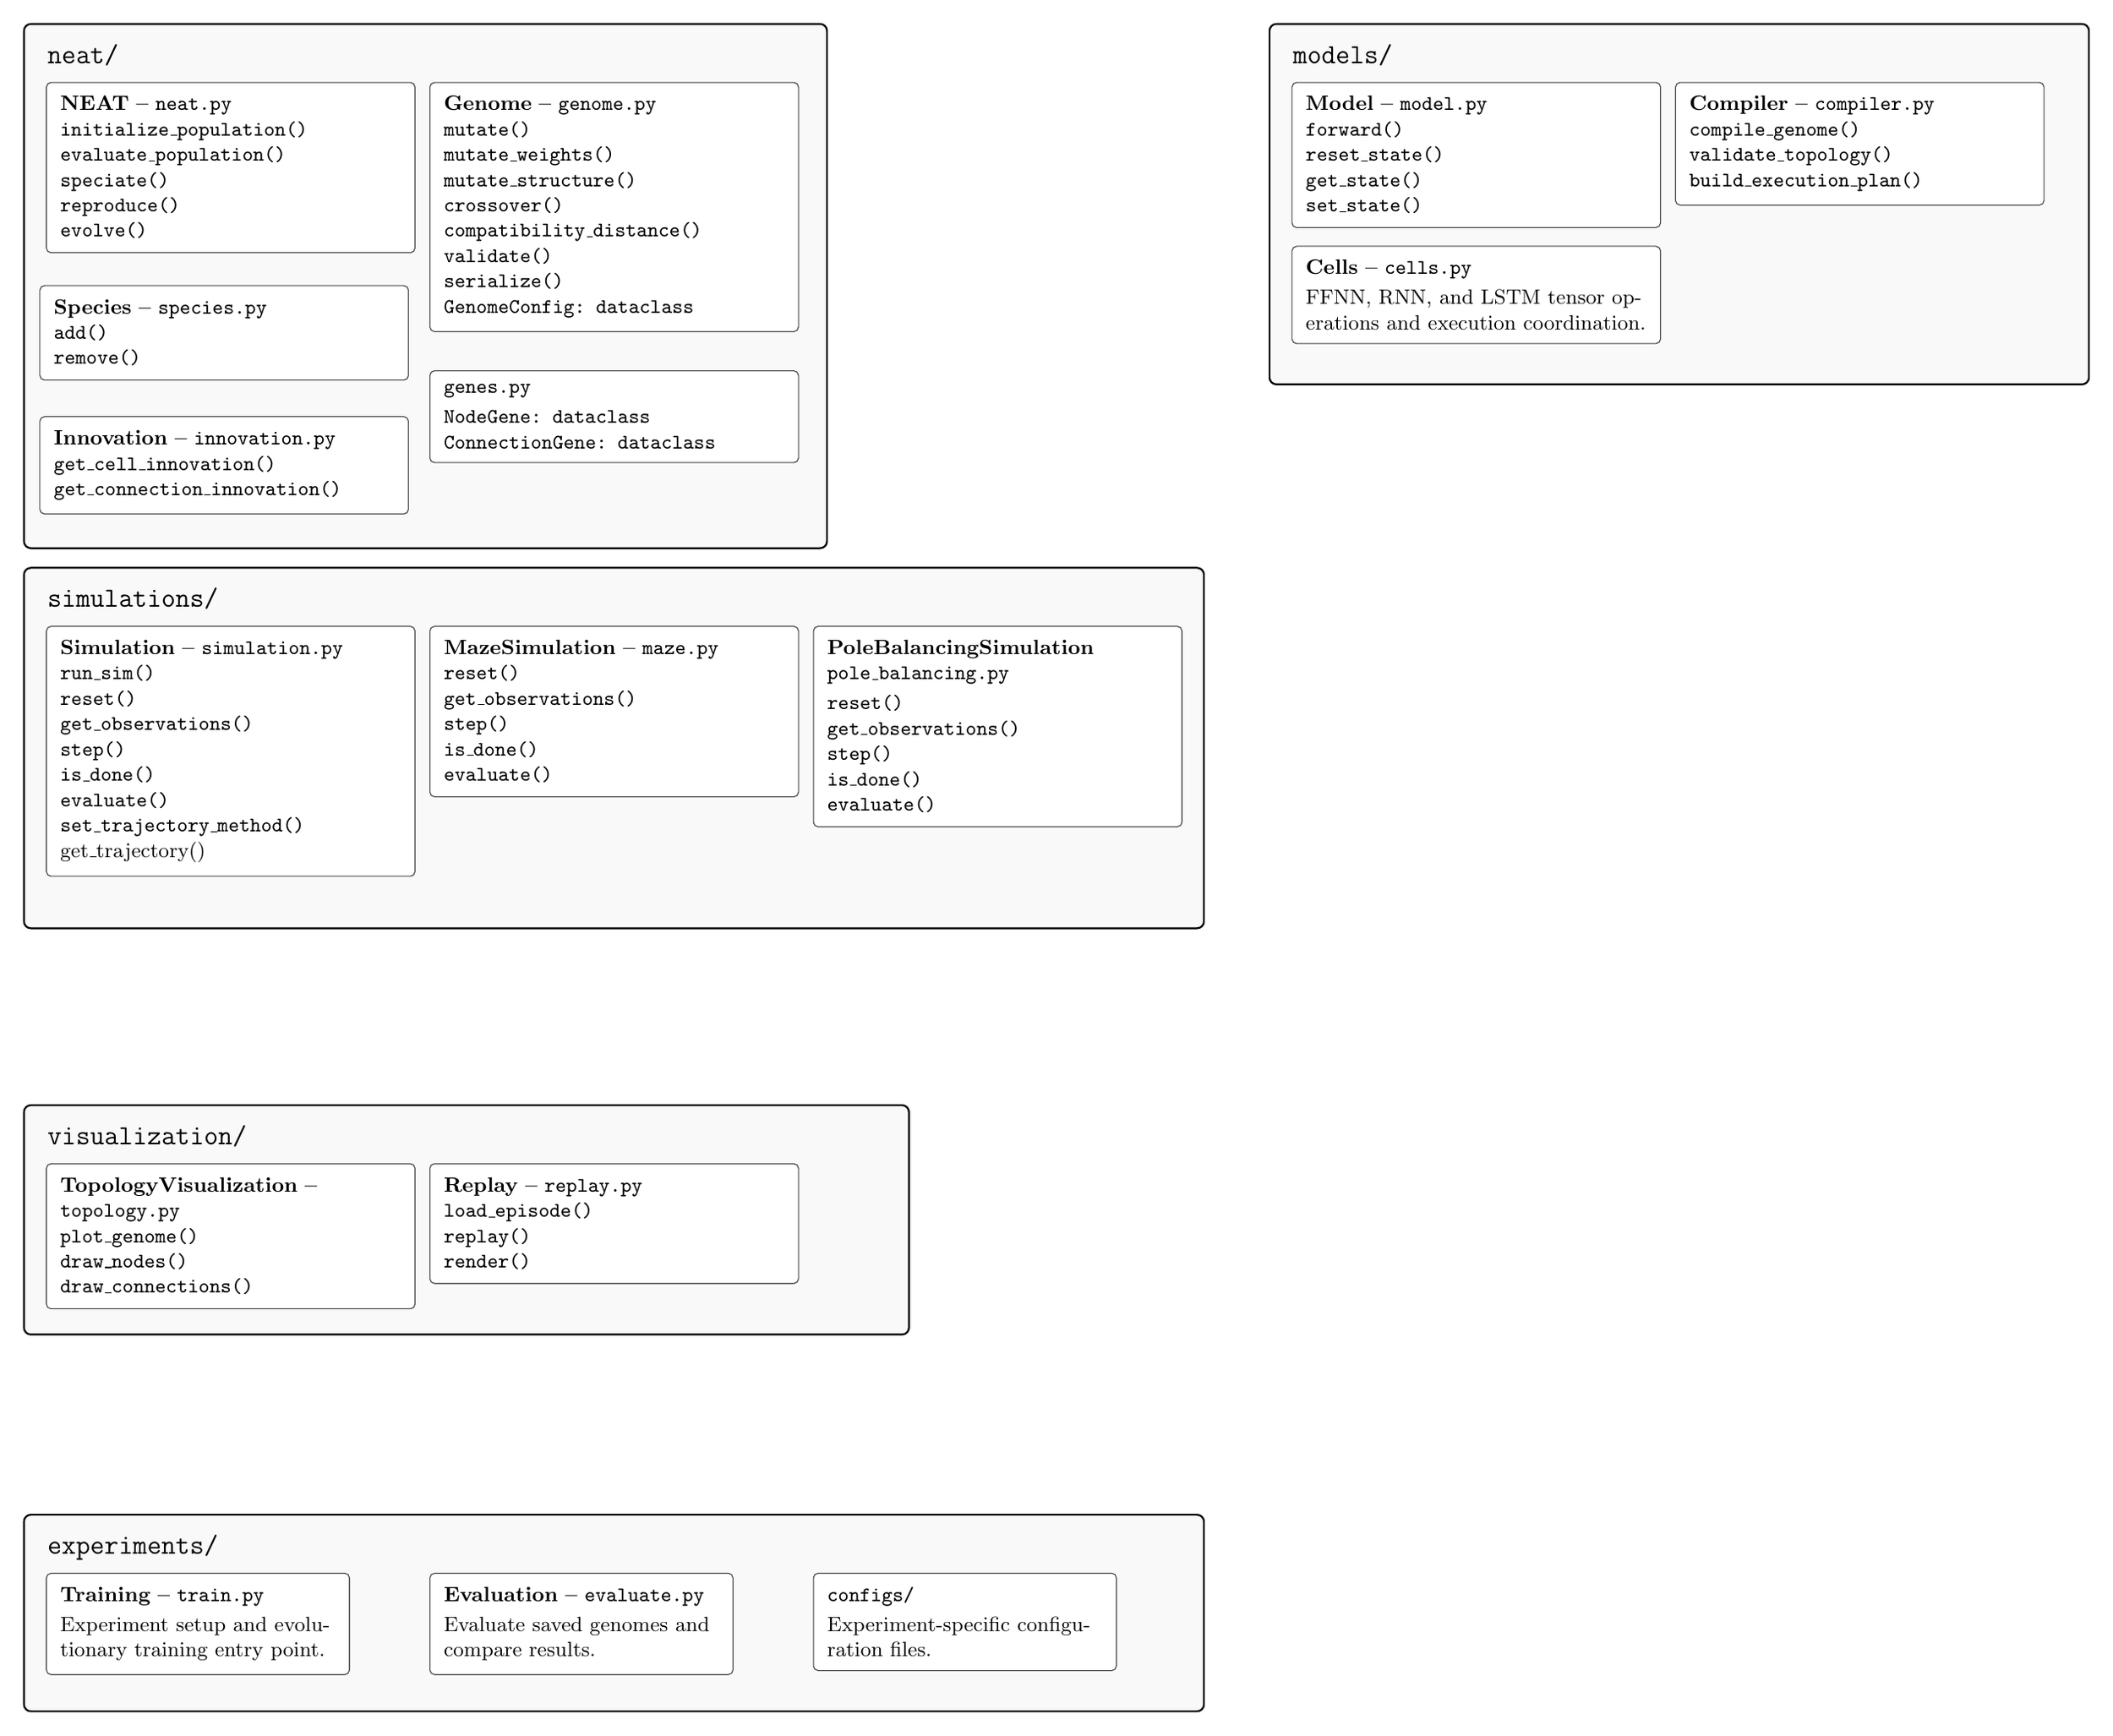
\begin{tikzpicture}[
    x=1cm,
    y=1cm
]

% ------------------------------------------------------------
% neat/
% ------------------------------------------------------------

\node[package, minimum width=12.25cm, minimum height=8.0cm,
      anchor=north west] (neatpkg) at (0,0) {};

\node[package title]
    at ([xshift=0.25cm,yshift=-0.2cm]neatpkg.north west)
    {\texttt{neat/}};

\node[wideclassbox, anchor=north west] (neatclass)
    at ([xshift=0.35cm,yshift=-0.9cm]neatpkg.north west)
    {
        \textbf{NEAT -- \texttt{neat.py}}\\
        \texttt{initialize\_population()}\\
        \texttt{evaluate\_population()}\\
        \texttt{speciate()}\\
        \texttt{reproduce()}\\
        \texttt{evolve()}
    };

\node[wideclassbox, anchor=north west] (genomeclass)
    at ([xshift=6.2cm,yshift=-0.9cm]neatpkg.north west)
    {
        \textbf{Genome -- \texttt{genome.py}}\\
        \texttt{mutate()}\\
        \texttt{mutate\_weights()}\\
        \texttt{mutate\_structure()}\\
        \texttt{crossover()}\\
        \texttt{compatibility\_distance()}\\
        \texttt{validate()}\\
        \texttt{serialize()}\\
        \texttt{GenomeConfig: dataclass}
    };

\node[wideclassbox, anchor=north west] (speciesclass)
    at ([xshift=0.25cm,yshift=-4.0cm]neatpkg.north west)
    {
        \textbf{Species -- \texttt{species.py}}\\
        \texttt{add()}\\
        \texttt{remove()}\\
    };

\node[wideclassbox, anchor=north west] (innovationclass)
    at ([xshift=0.25cm,yshift=-6.0cm]neatpkg.north west)
    {
        \textbf{Innovation -- \texttt{innovation.py}}\\
        \texttt{get\_cell\_innovation()}\\
        \texttt{get\_connection\_innovation()}\\
    };

\node[wideclassbox, anchor=north west] (genesclass)
    at ([xshift=6.2cm,yshift=-5.3cm]neatpkg.north west)
    {
        \texttt{genes.py}\\[2pt]
        \texttt{NodeGene: dataclass}\\
        \texttt{ConnectionGene: dataclass}\\
    };

% ------------------------------------------------------------
% models/
% ------------------------------------------------------------

\node[package, minimum width=12.5cm, minimum height=5.5cm,
      anchor=north west] (modelpkg) at (19.0,0) {};

\node[package title]
    at ([xshift=0.25cm,yshift=-0.2cm]modelpkg.north west)
    {\texttt{models/}};

\node[wideclassbox, anchor=north west] (modelclass)
    at ([xshift=0.35cm,yshift=-0.9cm]modelpkg.north west)
    {
        \textbf{Model -- \texttt{model.py}}\\
        \texttt{forward()}\\
        \texttt{reset\_state()}\\
        \texttt{get\_state()}\\
        \texttt{set\_state()}
    };

\node[wideclassbox, anchor=north west] (compilerclass)
    at ([xshift=6.2cm,yshift=-0.9cm]modelpkg.north west)
    {
        \textbf{Compiler -- \texttt{compiler.py}}\\
        \texttt{compile\_genome()}\\
        \texttt{validate\_topology()}\\
        \texttt{build\_execution\_plan()}
    };

\node[wideclassbox, anchor=north west] (executionclass)
    at ([xshift=0.35cm,yshift=-3.4cm]modelpkg.north west)
    {
        \textbf{Cells -- \texttt{cells.py}}\\[2pt]
        FFNN, RNN, and LSTM
        tensor operations and
        execution coordination.
    };

% ------------------------------------------------------------
% simulations/
% ------------------------------------------------------------

\node[package, minimum width=18.0cm, minimum height=5.5cm,
      anchor=north west] (simpkg) at (0,-8.3) {};

\node[package title]
    at ([xshift=0.25cm,yshift=-0.2cm]simpkg.north west)
    {\texttt{simulations/}};

\node[wideclassbox, anchor=north west] (simulationclass)
    at ([xshift=0.35cm,yshift=-0.9cm]simpkg.north west)
    {
        \textbf{Simulation -- \texttt{simulation.py}}\\
        \texttt{run\_sim()}\\
        \texttt{reset()}\\
        \texttt{get\_observations()}\\
        \texttt{step()}\\
        \texttt{is\_done()}\\
        \texttt{evaluate()}\\
        \texttt{set\_trajectory\_method()}\\
        \text{get\_trajectory()}

    };

\node[wideclassbox, anchor=north west] (mazeclass)
    at ([xshift=6.2cm,yshift=-0.9cm]simpkg.north west)
    {
        \textbf{MazeSimulation -- \texttt{maze.py}}\\
        \texttt{reset()}\\
        \texttt{get\_observations()}\\
        \texttt{step()}\\
        \texttt{is\_done()}\\
        \texttt{evaluate()}
    };

\node[wideclassbox, anchor=north west] (poleclass)
    at ([xshift=12.05cm,yshift=-0.9cm]simpkg.north west)
    {
        \textbf{PoleBalancingSimulation}\\
        \texttt{pole\_balancing.py}\\[2pt]
        \texttt{reset()}\\
        \texttt{get\_observations()}\\
        \texttt{step()}\\
        \texttt{is\_done()}\\
        \texttt{evaluate()}
    };

% ------------------------------------------------------------
% visualization/
% ------------------------------------------------------------

\node[package, minimum width=13.5cm, minimum height=3.5cm,
      anchor=north west] (vizpkg) at (0,-16.5) {};

\node[package title]
    at ([xshift=0.25cm,yshift=-0.2cm]vizpkg.north west)
    {\texttt{visualization/}};

\node[wideclassbox, anchor=north west] (topologyclass)
    at ([xshift=0.35cm,yshift=-0.9cm]vizpkg.north west)
    {
        \textbf{TopologyVisualization -- \texttt{topology.py}}\\
        \texttt{plot\_genome()}\\
        \texttt{draw\_nodes()}\\
        \texttt{draw\_connections()}
    };

\node[wideclassbox, anchor=north west] (replayclass)
    at ([xshift=6.2cm,yshift=-0.9cm]vizpkg.north west)
    {
        \textbf{Replay -- \texttt{replay.py}}\\
        \texttt{load\_episode()}\\
        \texttt{replay()}\\
        \texttt{render()}
    };

% ------------------------------------------------------------
% experiments/
% ------------------------------------------------------------

\node[package, minimum width=18.0cm, minimum height=3.0cm,
      anchor=north west] (exppkg) at (0,-22.75) {};

\node[package title]
    at ([xshift=0.25cm,yshift=-0.2cm]exppkg.north west)
    {\texttt{experiments/}};

\node[classbox, anchor=north west] (trainclass)
    at ([xshift=0.35cm,yshift=-0.9cm]exppkg.north west)
    {
        \textbf{Training -- \texttt{train.py}}\\[2pt]
        Experiment setup and
        evolutionary training entry point.
    };

\node[classbox, anchor=north west] (evaluateclass)
    at ([xshift=6.2cm,yshift=-0.9cm]exppkg.north west)
    {
        \textbf{Evaluation -- \texttt{evaluate.py}}\\[2pt]
        Evaluate saved genomes
        and compare results.
    };

\node[classbox, anchor=north west] (experimentconfig)
    at ([xshift=12.05cm,yshift=-0.9cm]exppkg.north west)
    {
        \textbf{\texttt{configs/}}\\[2pt]
        Experiment-specific
        configuration files.
    };

\end{tikzpicture}
\end{landscape}

% ============================================================
% PAGE 2: CLASS RELATIONSHIPS
% ============================================================

\newpage

\begin{landscape}
\begin{center}
    {\LARGE\bfseries Class Relationships}

    \vspace{0.2cm}
    {\small Conceptual ownership, inheritance, and usage relationships}
\end{center}

\vspace{0.3cm}

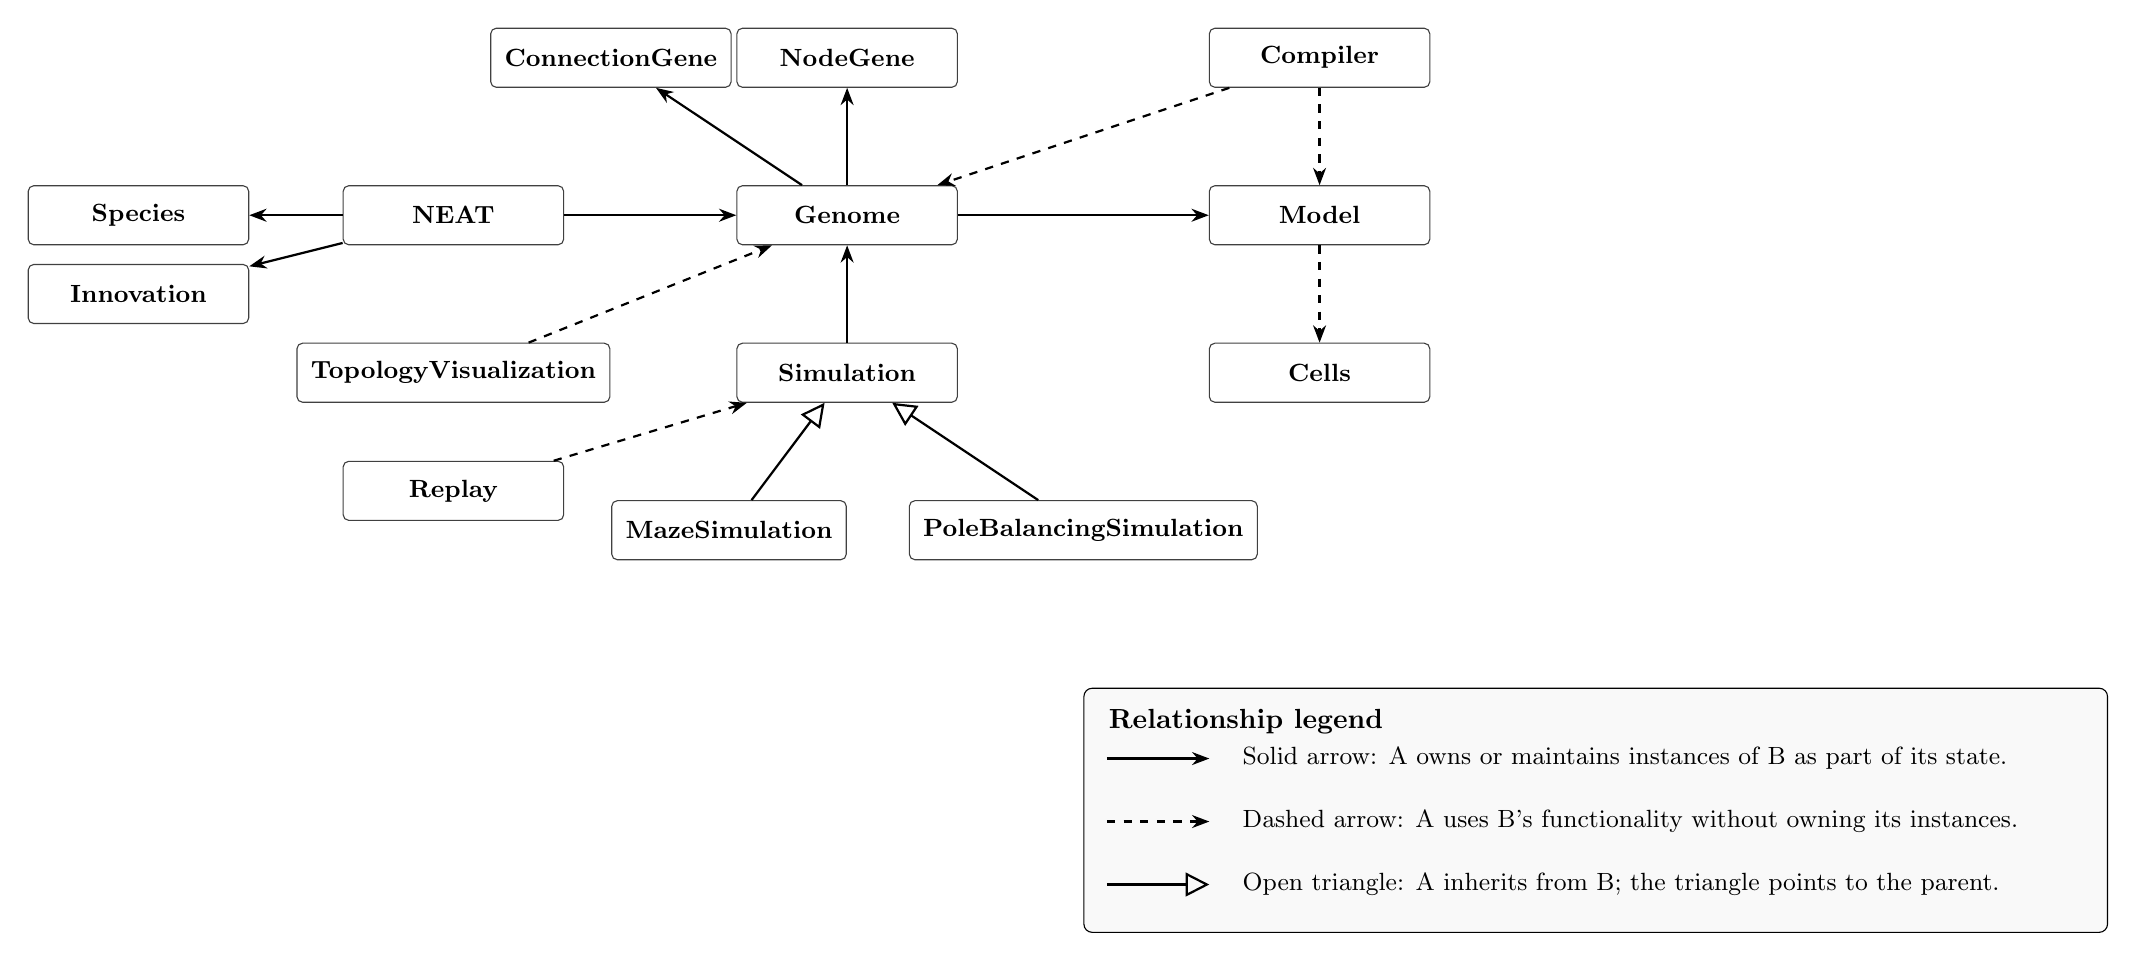
\begin{tikzpicture}[
    node distance=1.1cm and 1.2cm,
    every node/.style={font=\small},
    classnode/.style={
        draw=black!75,
        rounded corners=2pt,
        fill=white,
        align=center,
        font=\small\bfseries,
        minimum width=2.8cm,
        minimum height=0.75cm,
        inner sep=5pt
    },
    relation/.style={
        -{Stealth[length=2.2mm]},
        thick
    },
    dependency/.style={
        -{Stealth[length=2.2mm]},
        thick,
        dashed
    },
    inheritance/.style={
        -{Triangle[open,length=3mm,width=3mm]},
        thick
    }
]

% ------------------------------------------------------------
% NEAT ownership structure
% ------------------------------------------------------------

\node[classnode] (neat) at (2,-6) {NEAT};

\node[classnode] (genome) at (7,-6.0) {Genome};
\node[classnode] (species) at (-2,-6.0) {Species};
\node[classnode] (tracker) at (-2,-7.0) {Innovation};

\node[classnode] (nodegene) at (7,-4.0) {NodeGene};
\node[classnode] (connectiongene) at (4,-4) {ConnectionGene};

\draw[relation] (neat) -- (genome);
\draw[relation] (neat) -- (species);
\draw[relation] (neat) -- (tracker);

\draw[relation] (genome) -- (nodegene);
\draw[relation] (genome) -- (connectiongene);

% ------------------------------------------------------------
% Model compilation and execution
% ------------------------------------------------------------

\node[classnode] (compiler) at (13,-4) {Compiler};
\node[classnode] (model) at (13,-6.0) {Model};
\node[classnode] (execution) at (13,-8.0) {Cells};

\draw[dependency] (compiler) -- (genome);
\draw[relation] (genome) -- (model);
\draw[dependency] (compiler) -- (model);
\draw[dependency] (model) -- (execution);

% ------------------------------------------------------------
% Simulation and results
% ------------------------------------------------------------

\node[classnode] (simulation) at (7,-8.0) {Simulation};
\node[classnode] (maze) at (5.5,-10.0) {MazeSimulation};
\node[classnode] (pole) at (10,-10.0) {PoleBalancingSimulation};

\draw[inheritance] (maze) -- (simulation);
\draw[inheritance] (pole) -- (simulation);


% ------------------------------------------------------------
% Visualization
% ------------------------------------------------------------

\node[classnode] (topology) at (2,-8.0) {TopologyVisualization};
\node[classnode] (replay) at (2,-9.5) {Replay};

\draw[dependency] (topology) -- (genome);
\draw[dependency] (replay) -- (simulation);
\draw[relation] (simulation) -- (genome);

% ------------------------------------------------------------
% Boxed legend
% ------------------------------------------------------------

\node[
    draw=black,
    rounded corners=3pt,
    fill=gray!5,
    anchor=north west,
    minimum width=13.0cm,
    minimum height=3.1cm,
    inner sep=9pt
] (legend) at (10,-12.0) {};

\node[
    anchor=north west,
    font=\bfseries
] at ([xshift=0.2cm,yshift=-0.15cm]legend.north west)
    {Relationship legend};

\draw[relation]
    ([xshift=0.3cm,yshift=-0.9cm]legend.north west)
    -- ++(1.3cm,0);

\node[anchor=west,align=left]
    at ([xshift=1.9cm,yshift=-0.9cm]legend.north west)
    {Solid arrow: A owns or maintains instances of B as part of its state.};

\draw[dependency]
    ([xshift=0.3cm,yshift=-1.7cm]legend.north west)
    -- ++(1.3cm,0);

\node[anchor=west,align=left]
    at ([xshift=1.9cm,yshift=-1.7cm]legend.north west)
    {Dashed arrow: A uses B's functionality without owning its instances.};

\draw[inheritance]
    ([xshift=0.3cm,yshift=-2.5cm]legend.north west)
    -- ++(1.3cm,0);

\node[anchor=west,align=left]
    at ([xshift=1.9cm,yshift=-2.5cm]legend.north west)
    {Open triangle: A inherits from B; the triangle points to the parent.};

\end{tikzpicture}
\end{landscape}

\end{document}